\section*{Debt}

\subsection*{Create new debt}

\begin{itemize}
  \item[] \textbf{Trigger:} User interaction with CMS window
  \item[] \textbf{Precondition:} Assert that user has logged in
  \item[] \textbf{Path:}
    \begin{enumerate}
      \item User clicks Admin on navigation bar
      \item User clicks on Debts in the dropdown
      \item User clicks ``New Debt'' button
      \item User fills the debt information in the form
      \item User clicks ``Create Debt'' button
      \item ``Debt successfully created'' message is shown together with the data
    \end{enumerate}
  \item[] \textbf{Requirements:}
    \begin{enumerate}
      \item The new debt's data should be added to the database
      \item The new debt's information should be displayed in the homepage correctly
      \item The debts' information should be listed in the creation order
    \end{enumerate}
  \item[] \textbf{Screenshots:} \\
    \includegraphics[scale=0.25]{./images/ss/debt/create/1.png}
    \includegraphics[scale=0.25]{./images/ss/debt/create/2.png}\\
    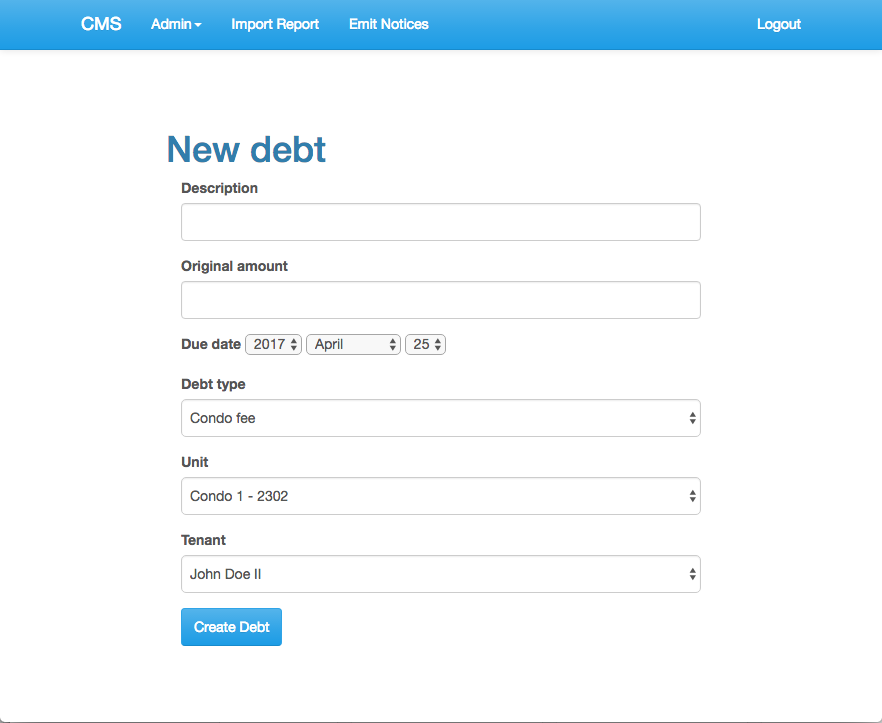
\includegraphics[scale=0.25]{./images/ss/debt/create/3.png}
    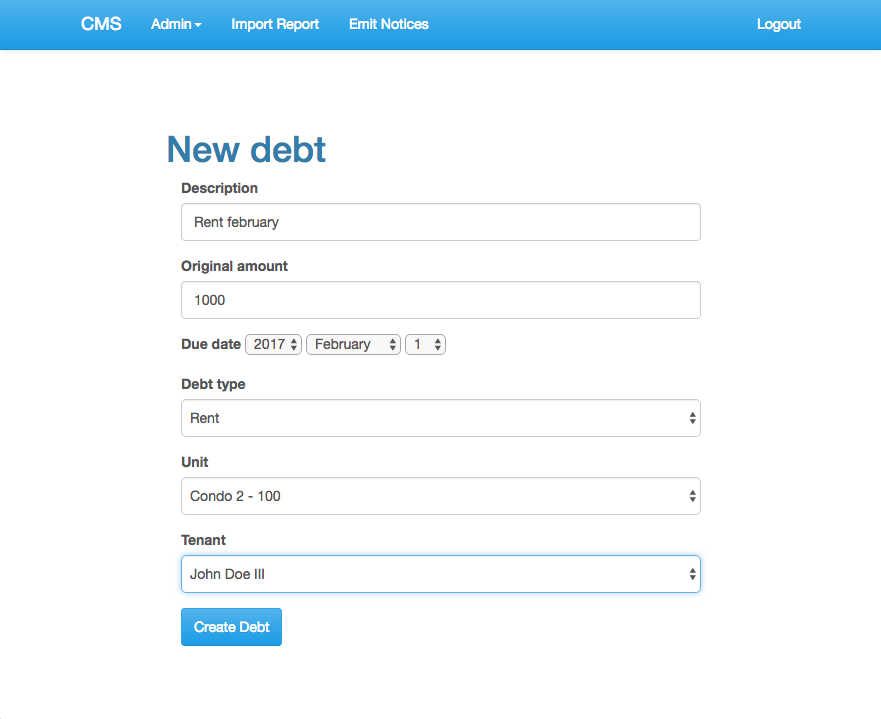
\includegraphics[scale=0.25]{./images/ss/debt/create/4.png}\\
    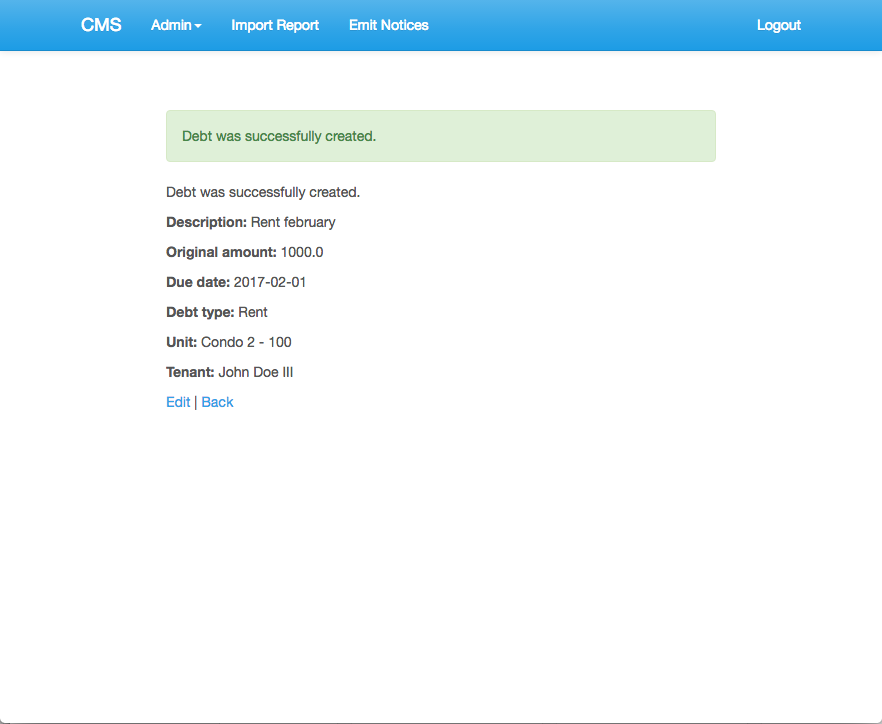
\includegraphics[scale=0.25]{./images/ss/debt/create/5.png}
\end{itemize}

\subsection*{Edit a debt}

\begin{itemize}
  \item[] \textbf{Trigger:} User interaction with CMS window
  \item[] \textbf{Precondition:} Assert that user is in the Debt page and the debt to edit is existed
  \item[] \textbf{Path:}
    \begin{enumerate}
      \item User clicks on Edit behind the information of the debt who will be edited
      \item User edit new information in the form
      \item User clicks ``Update Debt'' button
      \item ``Debt successfully updated'' massage is shown
    \end{enumerate}
  \item[] \textbf{Requirements:}
    \begin{enumerate}
      \item The updated debt’s new data should be updated to the database
      \item The updated debt’s new information should be displayed in the homepage correctly
      \item The debts’ information should be listed in the modification order
    \end{enumerate}
  \item[] \textbf{Screenshots:}\\
    \includegraphics[scale=0.25]{./images/ss/debt/edit/1.png}
    \includegraphics[scale=0.25]{./images/ss/debt/edit/2.png}\\
    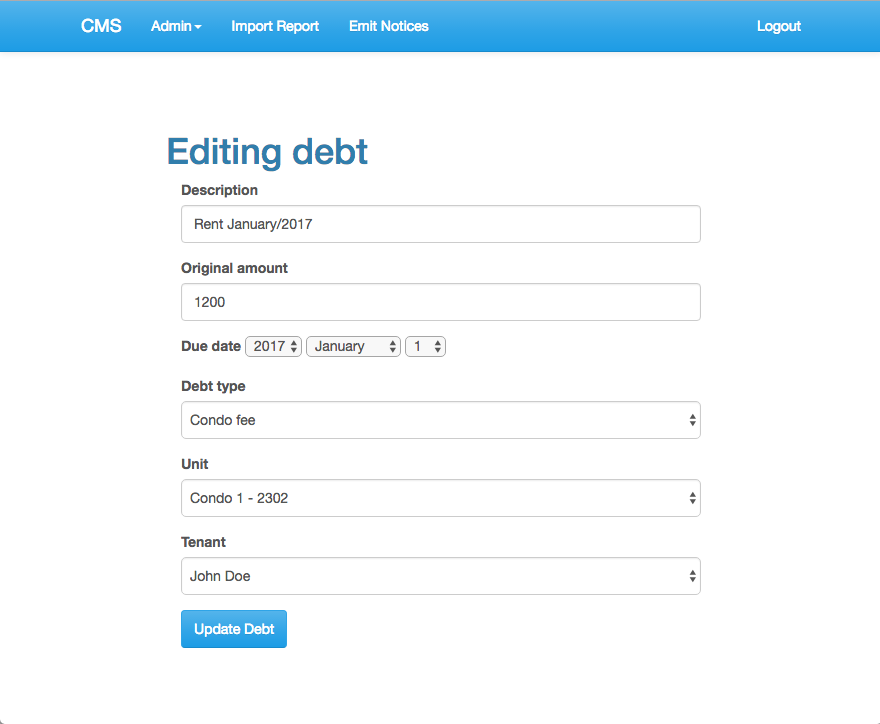
\includegraphics[scale=0.25]{./images/ss/debt/edit/3.png}
    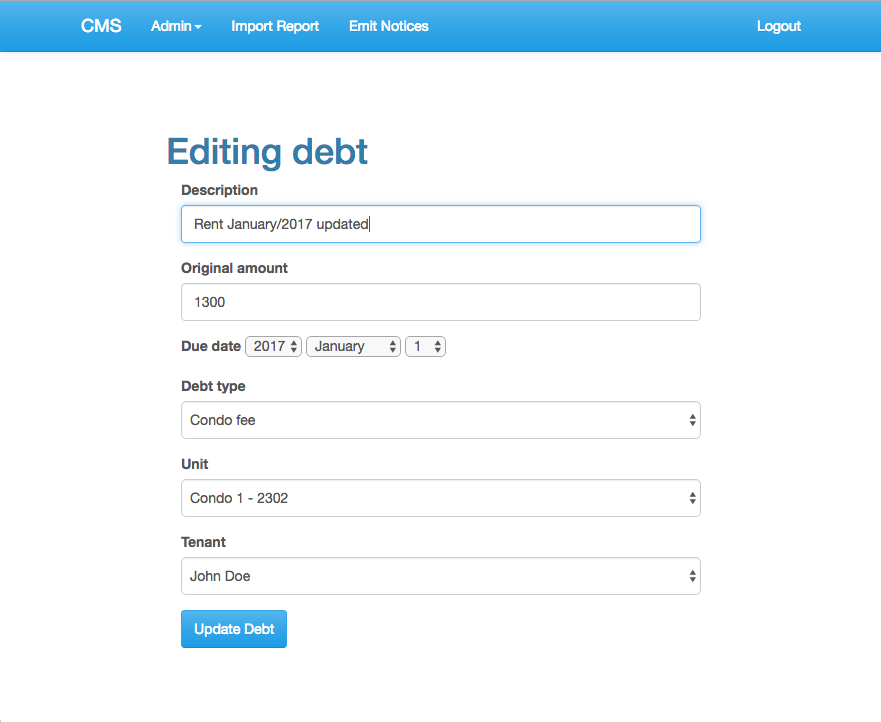
\includegraphics[scale=0.25]{./images/ss/debt/edit/4.png}\\
    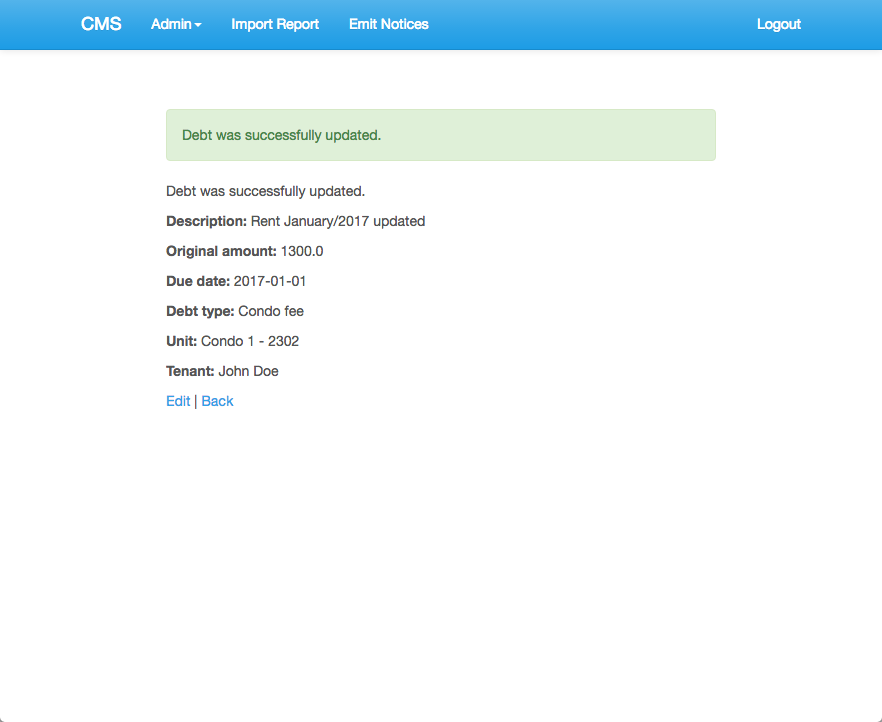
\includegraphics[scale=0.25]{./images/ss/debt/edit/5.png}
\end{itemize}

\subsection*{Delete a debt}

\begin{itemize}
  \item[] \textbf{Trigger:} User interaction with CMS window
  \item[] \textbf{Precondition:} Assert that user is in the Debt page and the debt to edit is existed
  \item[] \textbf{Path:}
    \begin{enumerate}
      \item User clicks on Destroy at the end of the information of the debt who will be deleted
      \item An alter message says ``Are you sure'' is shown
      \item User clicks ``OK'' button
      \item Debt successfully destroyed massage is shown
    \end{enumerate}
  \item[] \textbf{Requirements:}
    \begin{enumerate}
      \item The deleted debt’s data should be removed to the database
      \item The deleted debt’s information should not be displayed in the homepage
      \item Other debts’ information should be listed as the same as those before deleting
    \end{enumerate}
  \item[] \textbf{Screenshots:}\\
    \includegraphics[scale=0.25]{./images/ss/debt/delete/1.png}
    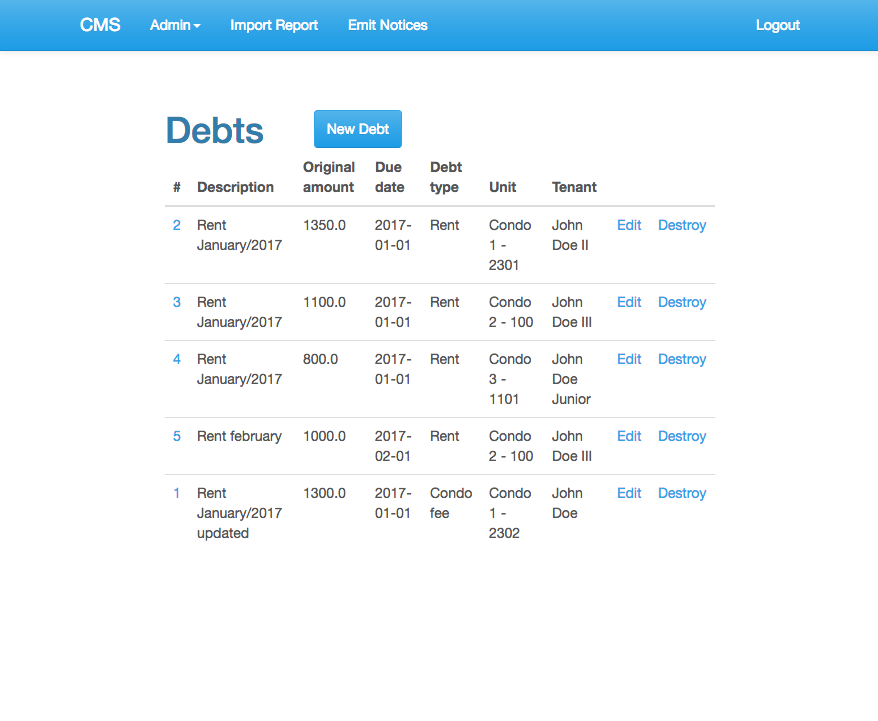
\includegraphics[scale=0.25]{./images/ss/debt/delete/2.png}\\
    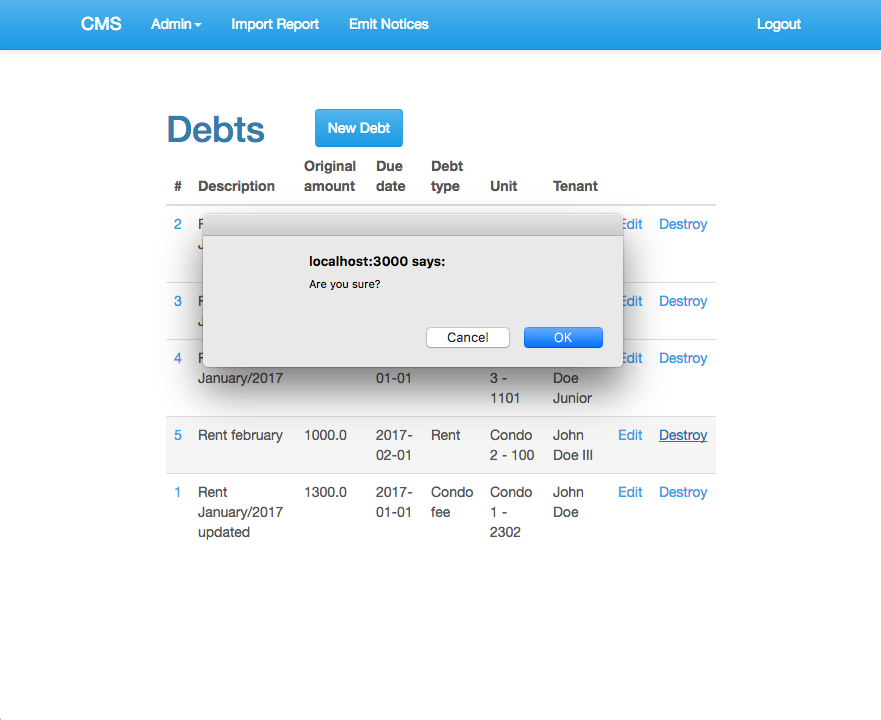
\includegraphics[scale=0.25]{./images/ss/debt/delete/3.png}
    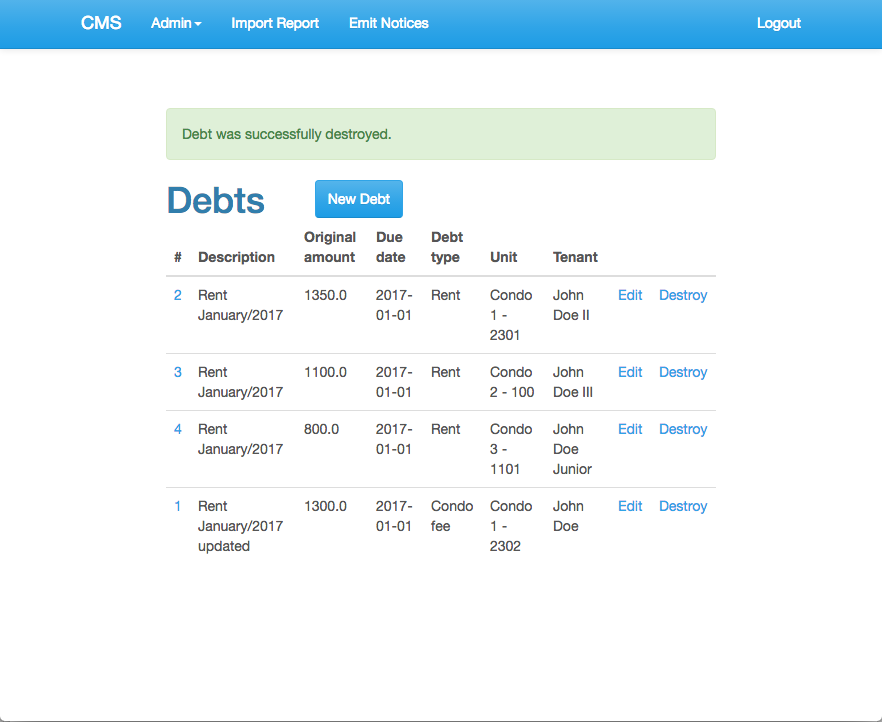
\includegraphics[scale=0.25]{./images/ss/debt/delete/4.png}
\end{itemize}
